
% ---------------------------- comment out when compiling the full document -------------------
\documentclass[11pt]{mytustyle}  % default square logo 
\usepackage{amssymb}
\usepackage{caption}
\usepackage{upgreek}
\usepackage{subfig}

\usepackage{packages/fancyhdr}% http://ctan.org/pkg/fancyhdr
\pagestyle{fancy}% Change page style to fancy
%\fancyhf{}% Clear header/footer
\fancyhead{}
\fancyhead[RO, LE]{Experimental results}
%\fancyfoot{}
%\fancyfoot[RO, LE]{\thepage}% \fancyfoot[R]{\thepage}
\renewcommand{\headrulewidth}{0.7pt}% Default \headrulewidth is 0.4pt
%\renewcommand{\footrulewidth}{0.7pt}% Default \footrulewidth is 0pt
%\rfoot{\thepage}

\begin{document}
\baselineskip=16pt
% ---------------------------------------------------------------------------------------------------------------


% ---------------------------------------------------------------------------------------------------------------
\chapter{Experimental results}
% ---------------------------------------------------------------------------------------------------------------

Noise limitations

Lab measurements

Temperature and radiation limitations

Transient current technique

Charge - before and after irradiation

compare with RD42 results

Generation of trapping centres, reference KIT, Marok, Harris�

IIa



This chapter contains the measurement results of data taken with diamond sensors. The description of measurement setup (section~\ref{sec:meassetup}) and the experimental technique (section~\ref{sec:exptech}) is followed by discussion of limitations in sections \ref{sec:noiselimit}, \ref{sec:templimit} and \ref{sec:radlimit}. The aim of the chapter is to compare the experimentally acquired data with the theory from the previous chapter. 

% ---------------------------------------------------------------------------------------------------------------
\clearpage
\section{Measurement setup}
\label{sec:meassetup}
% ---------------------------------------------------------------------------------------------------------------

The measurement chain consists of three main parts: a diamond sensor, a signal preamplifier and a readout device, as seen in diagram~\ref{fig:ro-chain}. 

The signals propagating along the analogue chain are fast and with low amplitudes, which gives rise to importance of RF shielding. For instance, the sensor carrier has to be RF-tight to shield from external interferences. Also, the connection between the carrier and the preamplifier has to be as short as possible to avoid capacitive signal losses in the transmission line. Finally, the system needs to be grounded properly.

\begin{figure}
\centering
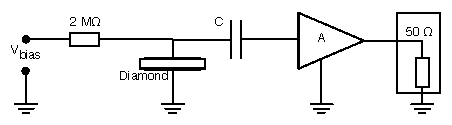
\includegraphics[width=0.8\textwidth]{plots/ro-chain}
\caption{Diagram of a diamond detector readout chain.}
\label{fig:ro-chain}
\end{figure}


\subsection{Preamplifiers}
\label{sec:preamps}
Two preamplifiers were used for the measurements, both embedded in an RF-tight aluminium box to reduce the noise pickup. Both have an AC coupled input and a 50~$\Upomega$ output.

\emph{CIVIDEC C2} is a fast current preamplifier with a 2~GHz bandwidth limit. It is used for TCT measurements because if its fast response and a good SNR.

\emph{CIVIDEC Cx} is a charge shaping amplifier. Its high SNR (low noise of 400~electrons and gain of 8.2~mV/fC) makes it a good choice for spectroscopic measurements with diamond sensors.

\begin{figure}[!ht]
%\centering
\begin{tabular}{cccc}
\subfloat[Cx charge shaping preamplifier]{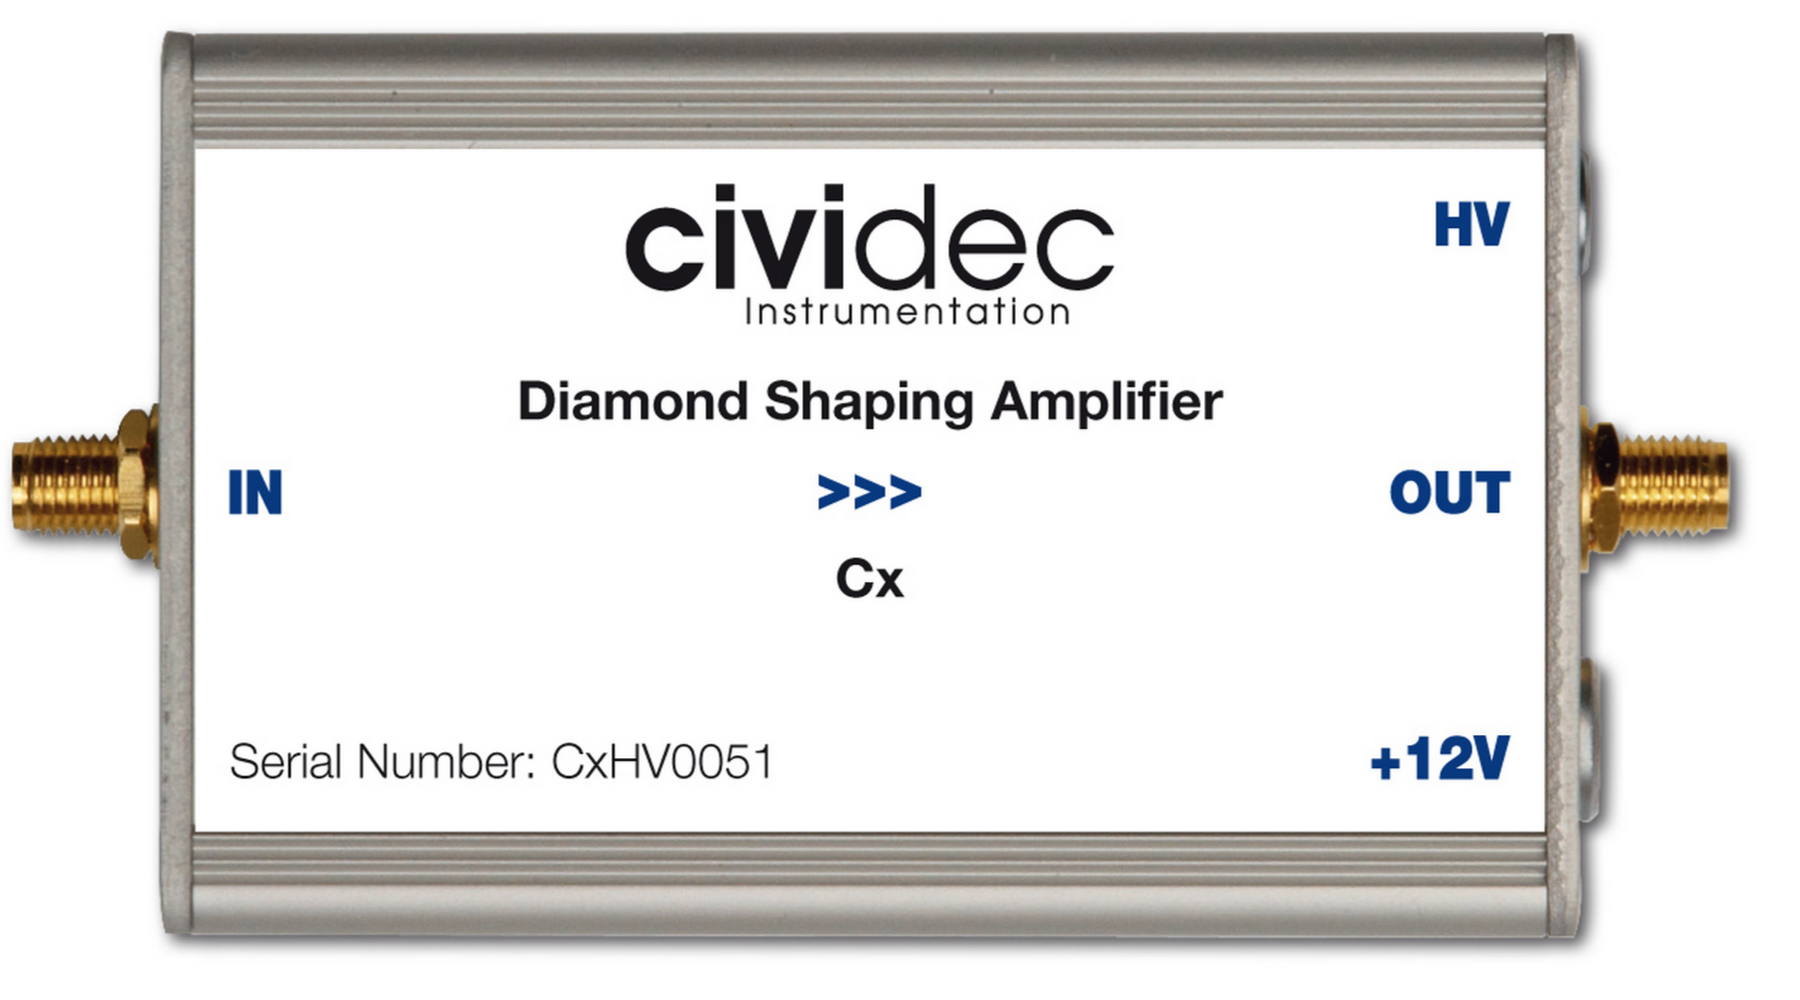
\includegraphics[width=0.45\textwidth]{pics/setup/Cx} \label{fig:ampcx}} &
\subfloat[C2 fast charge preamplifier]{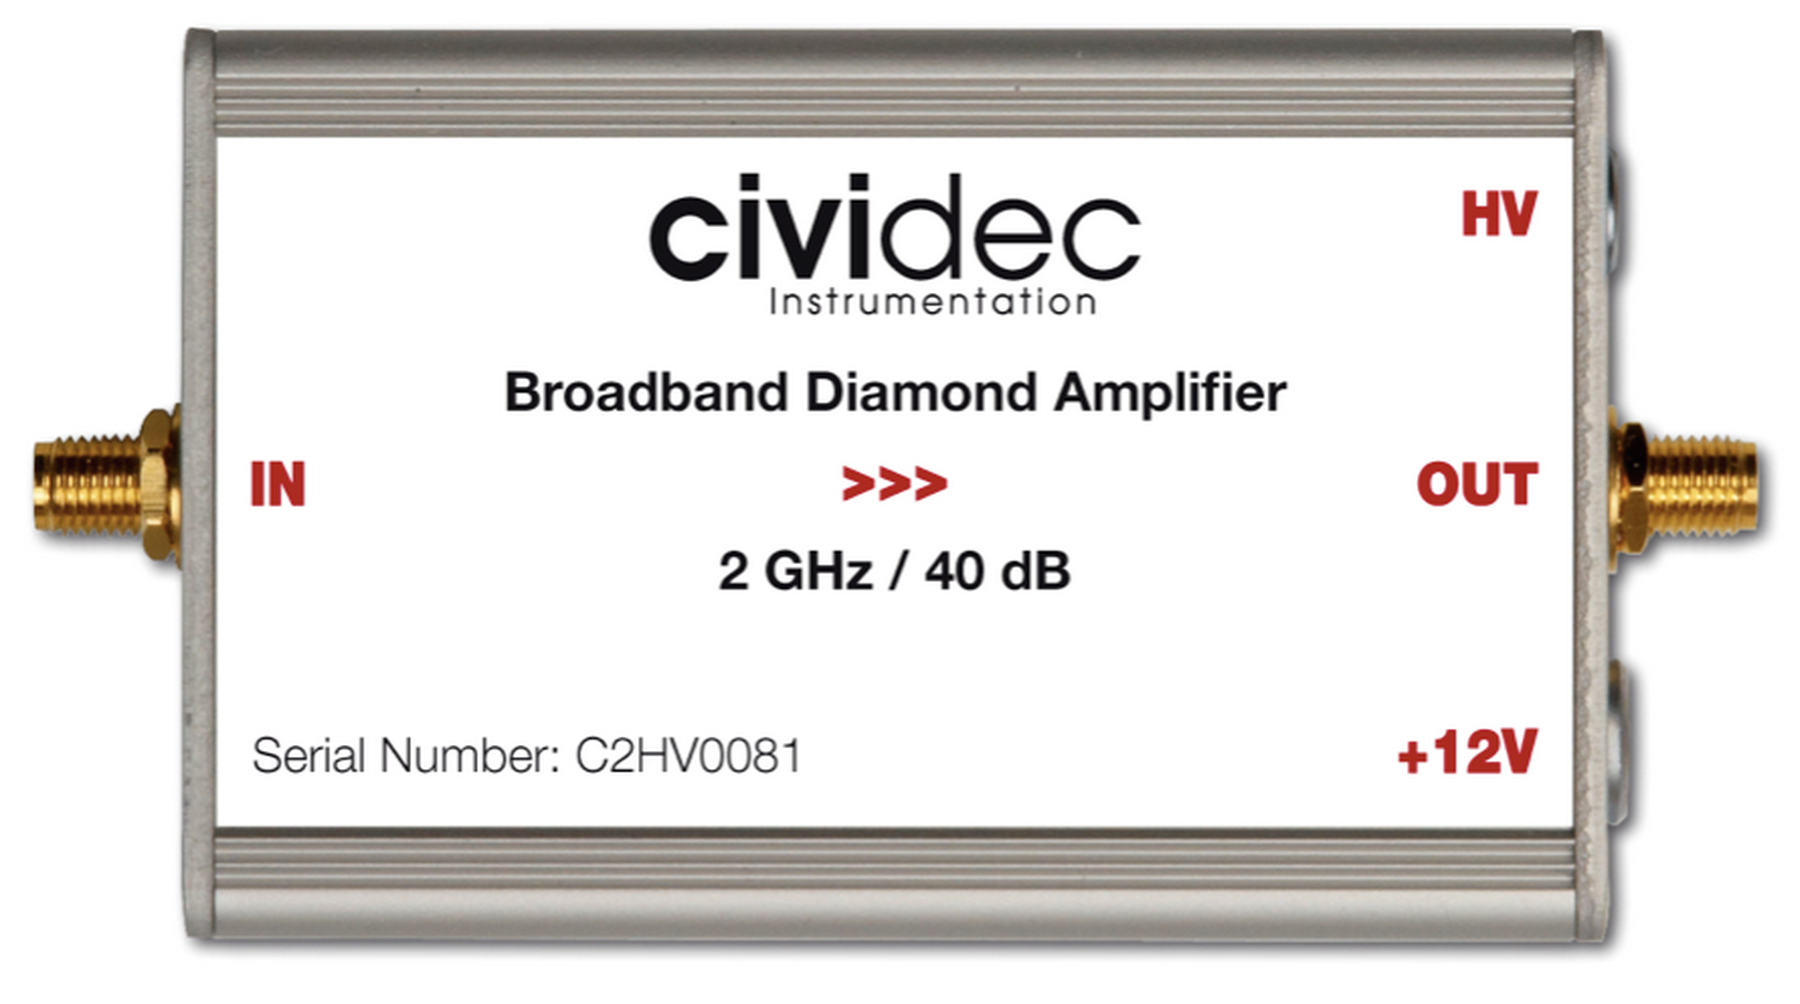
\includegraphics[width=0.45\textwidth]{pics/setup/C2}  \label{fig:ampc2}}
\end{tabular}
\caption{Thermal neutron measurement setup}
\end{figure}


\subsubsection{Diamond samples}
\label{sec:diamsam}


\begin{footnotesize}
\begin{center}
\captionof{table}{Diamond sensor samples used}
\begin{tabular}{   l  c  c  c c }
\hline
Name & Producer & Dimensions (x, y) [mm$^2$] & Thickness [$\upmu$m] & Irradiatied \\
\hline
S37 & E6 & $4.7\times4.7$ & 548 & no \\
S50 & E6 & $4.7\times4.7$ & 537 & no \\
S52 & E6 & $4.7\times4.7$ & 515 & $1\times10^{14}~p/cm^{-2}$ \\
S79 & E6 & $4.7\times4.7$ & 529 & $3.63\times10^{14}~p/cm^{-2}$ \\
ELSC & E6 & $4.7\times4.7$ & 491 & no \\
1scdhq & IIa & $5.6\times5.3$ & 460 & no \\
\hline
\end{tabular}
\label{tab:diamsamp}
\end{center}
\end{footnotesize}



\begin{figure}
\centering
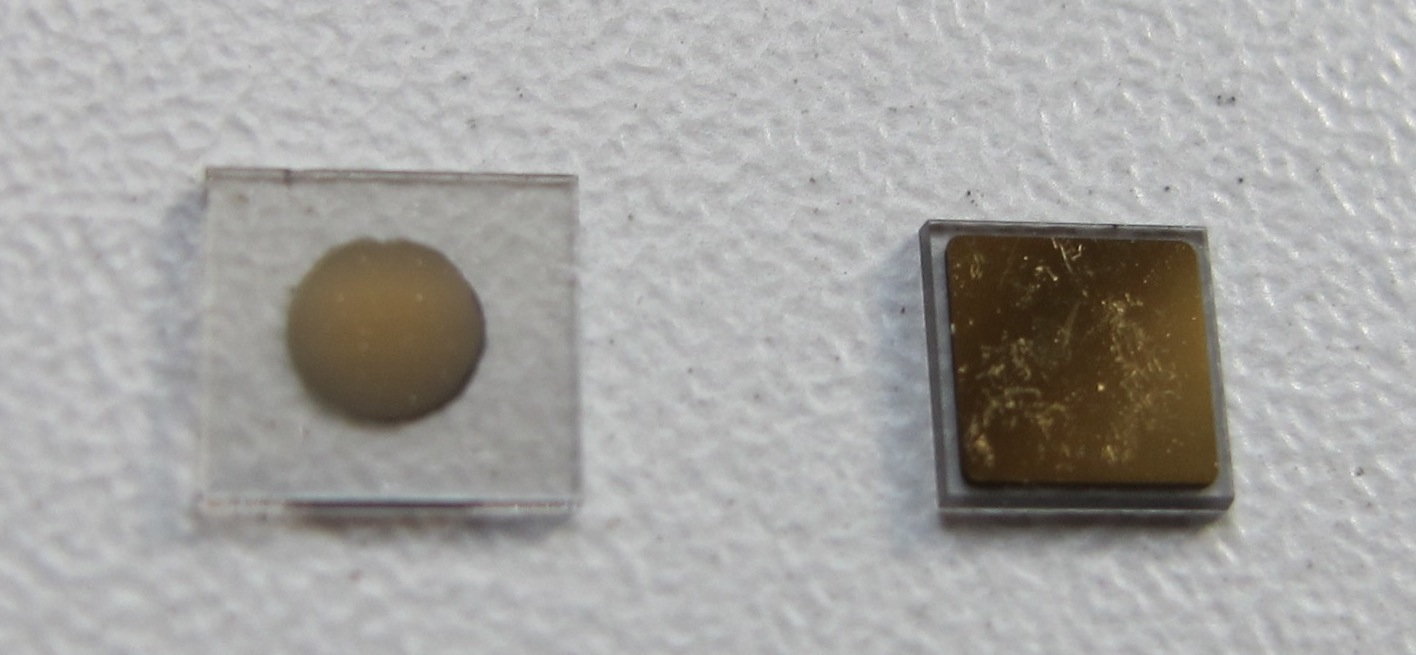
\includegraphics[width=0.8\textwidth]{pics/setup/diamond4}
\caption{Two scCVD diamond samples: A IIa 1scdhq (size $5.3\times5.6\times0.460~mm^3$) and a E6 S37 (dimensions $4.7\times4.7\times0.548~mm^3$)}
\label{fig:diams}
\end{figure}



\subsubsection{Readout device}
\label{sec:readoutdev}
Oscilloscopes are the most versatile analogue signal readout devices - fast to set up and reliable. It is important, though, to choose an oscilloscope with high enough bandwidth, especially for the fast current preamplifier signals. The choice for this setup was a 1~GHz and a 2~GHz option from the LeCroy WaveRunner family.

\subsection{Cryogenic setup}
\label{sec:cryosetup}


\begin{figure}[!ht]
%\centering
\begin{tabular}{cccc}
\subfloat[Sensor carrier]{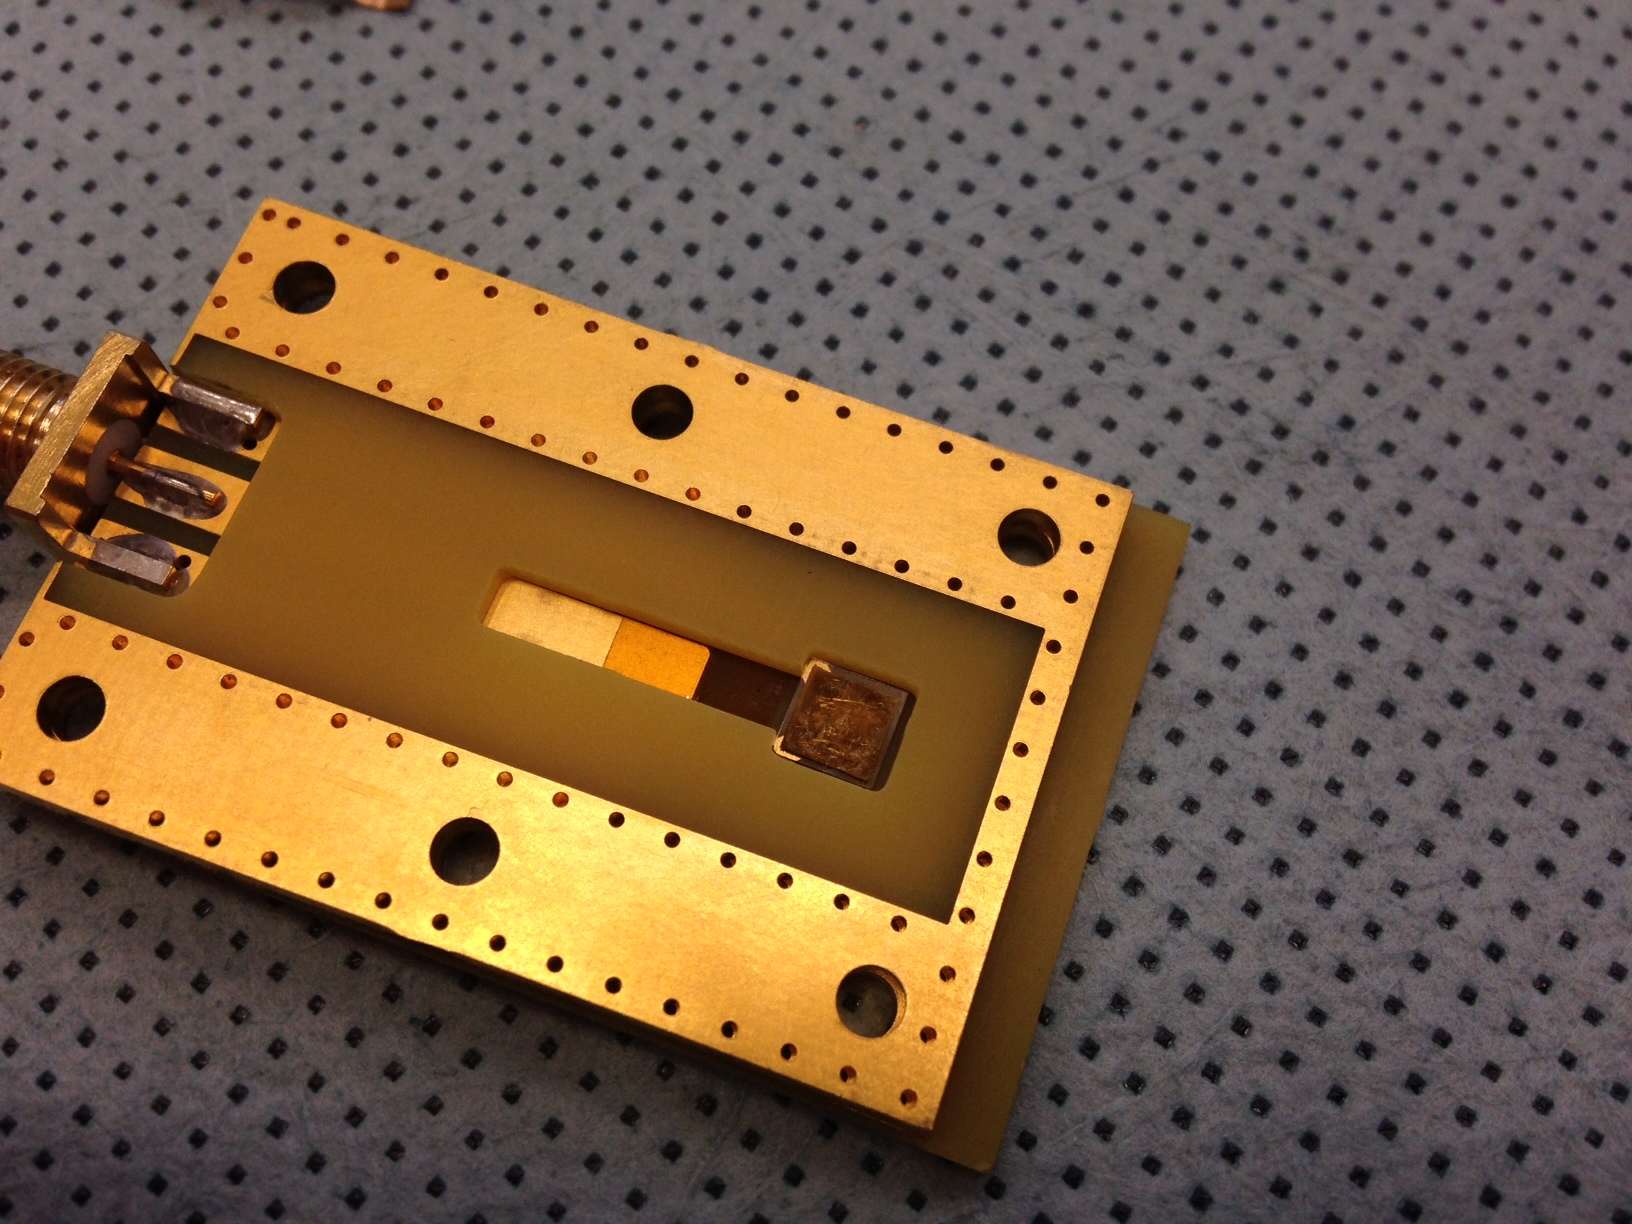
\includegraphics[width=0.45\textwidth]{pics/setup/carrier2} \label{fig:carrier}} &
\subfloat[Radioactive source]{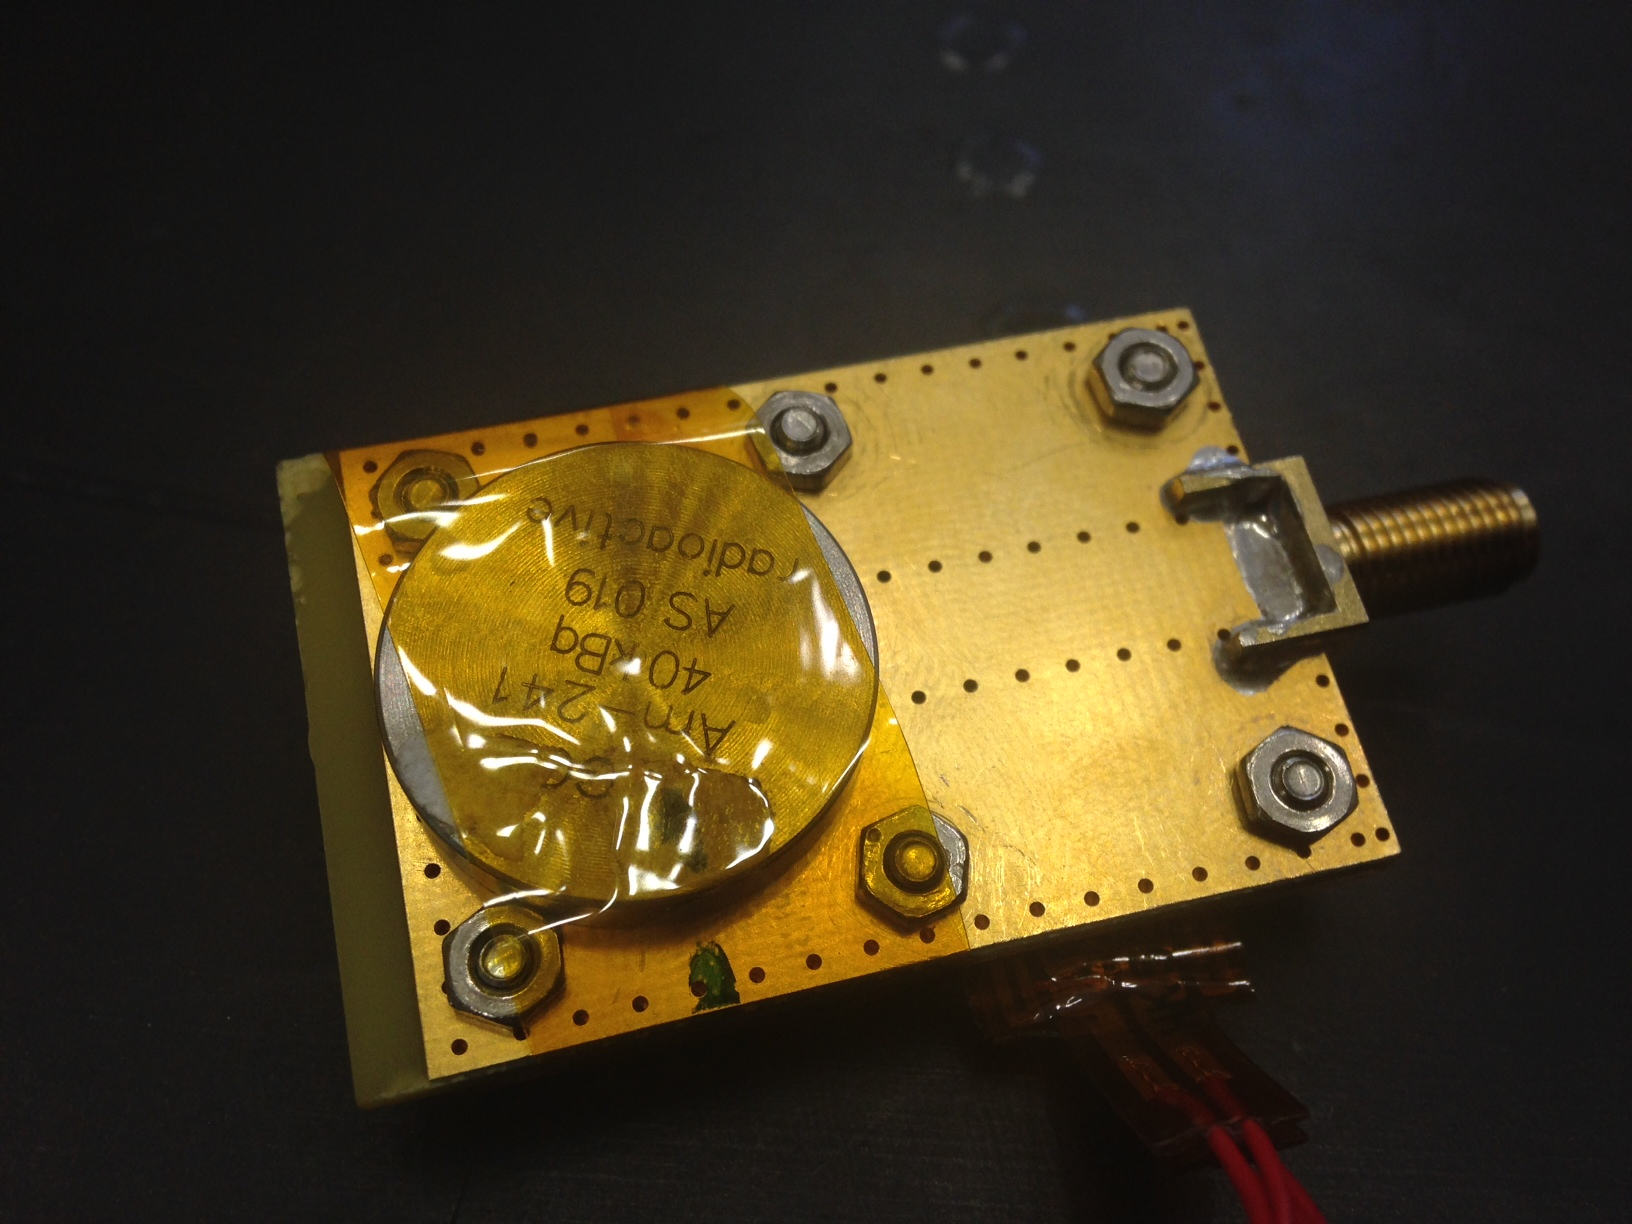
\includegraphics[width=0.45\textwidth]{pics/setup/carriersource2}  \label{fig:carsrc}}
\end{tabular}
\caption{Positioning of the $\alpha$-source on top of the sensor carrier}
\end{figure}







% ---------------------------------------------------------------------------------------------------------------
\clearpage
\section{Particle and photon pulses and spectra}
\label{sec:pulsespectra}
% ---------------------------------------------------------------------------------------------------------------


%\section{Pulse formation}
% ---------------------------------------------------------------------------------------------------------------
\clearpage
\section{Noise limitations}
\label{sec:noiselimit}
% ---------------------------------------------------------------------------------------------------------------
TO DO: Take 8 runs with the 2GHz oscilloscope while increasing the noise. 

Noise is a major limiting factor in particle detection. It defines the minimum measurable particle energy. It is hence important to 

% ---------------------------------------------------------------------------------------------------------------
\clearpage
\section{Temperature limitations}
\label{sec:templimit}
% ---------------------------------------------------------------------------------------------------------------
A test was carried out to evaluate the effect of temperature changes on the output signal of the diamond sensors. A cryostat filled with liquid helium was used to cool down the sensor during the measurement process. Current signal response to $\alpha$-particles was measured at $\sim$20 temperature points between 4~K and 295~K (room temperature - RT). At every temperature point, a set of 300 pulses was read out at various bias voltages. Resulting data showed that the charge collection is stable down to 150~K, where it starts decreasing and stabilises again at a third of the initial value at 75~K. This behaviour was first measured and discussed by H. Jansen in~\cite{JansenThesis}.

\subsection{Temperature-variant TCT}




% ---------------------------------------------------------------------------------------------------------------
\clearpage
\section{Radiation limitations}
\label{sec:radlimit}
% ---------------------------------------------------------------------------------------------------------------
Exposure to ionising radiation degrades sensors. It introduces so-called charge traps in the sensor material. The electrons and holes created by the impinging particle get trapped in these traps, decreasing the induced current on the electrodes. This yields a lower integrated charge in an irradiated sensor than that in a non-irradiated one. Charge collection efficiency is therefore correlated with the level of irradiation. In semiconductors, it follows an inverse exponential curve ?????

\subsection{Quantifying radiation damage in diamonds}
The last few decades have seen extensive efforts put into understanding and quantifying radiation damage in semiconductors. This varies with the type of radiation (particles or photons) and its energy. There are models existing that try to explain the impact of irradiation and to provide \emph{hardness factors} to compare the radiation damage between different particles. The standard way is to convert the damage into \emph{neutron equivalent}. Some models have been extensively verified with simulations and experimentally. In these experiments charge collection in sensors is measured before and after irradiation. This procedure is repeated several times, with a measurement point taken after every irradiation. When a set of measurements of charge collection is plotted against the radiation dose received by a specific particle at a specific , a damage factor $k_\lambda$ can be extracted. Damage factors across a range of energies and types of particles (photons) have to be measured to properly quantify the damage in the sensors. They are then compared against the simulations to verify that the experimental observations are in line with the theory.

Radiation damage in silicon, for instance, is well understood and explained. Silicon sensor is relatively cheap and widespread, which facilitated the irradiation experiments. Diamond, however, is an expensive material and the technology is relatively new as compared to silicon. Therefore not many institutes are carrying out diamond irradiation studies. To join the efforts, a collaboration called RD42 was formed. It gathers the experimental data from diamond irradiation studies. Unlike with silicon, the experimental results so far show no significant correlation with the NIEL (non-ionising energy loss) model~\cite{XXX}, which correlates detector efficiency with the \emph{number of lattice displacements}. Therefore an alternative model was proposed by Karlsruhe Institute of Technology~\cite{XXX}, correlating the diamond efficiency with \emph{displacements per atom} (DPA) in the bulk. Figure~\ref{fig:kitdpa} shows the DPA model for a range of energies of proton, pion and neutron irradiation in diamond. It has been normalised to damage in 24~GeV protons. According to the plot, a 300~MeV pion beam damages the diamond bulk twice as much as a 24~GeV proton beam.


\begin{figure}[!ht]
\begin{center}
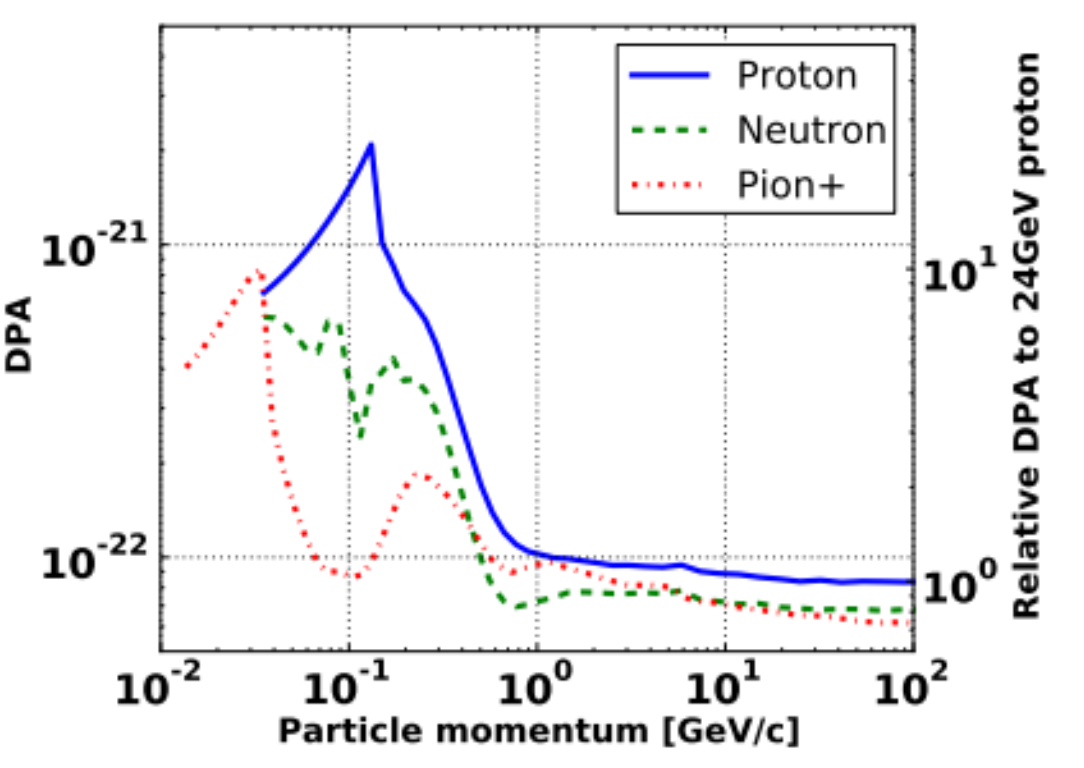
\includegraphics[width=0.6\textwidth]{plots/DPAplaceholder}
\caption{Diamond radiation damage - a model based on displacements per atom. Courtesy Karlsruhe Institute of Technology~\cite{} PLACEHOLDER}
\label{fig:kitdpa}
\end{center}
\end{figure}



\subsubsection{Pion irradiation}
Paul Scherrer Institute (PSI) is the largest research institute for material sciences in Switzerland. Among other they also carry out irradiation campaigns. Their 300~MeV/c (kinetic energy 191.31~MeV) pion beam with a flux of up to $1.5\times10^{14}~pions~cm^{-2}~day^{-1}$. Due to the uncertainty on the hardness factor, the equivalent fluences have an error of $\pm20~\%$.

Two diamond samples, S52 and S79, were exposed to the pion beam in the 2014 PSI irradiation campaign; S52 to $1\times10^{14}~pions~cm^{-2}$ and S79 to $3.63\times10^{14}~pions~cm^{-2}$. During the process, the golden electrodes got slightly activated, but the activation decayed in two weeks.

\subsubsection{Charge collection distance}
Three diamonds -- non-irradiated S37 and irradiated S52 and S79 -- were exposed to a 120~GeV test beam before and after irradiation to estimate the charge collection distance (CCD) and its decrease after irradiation. The samples were "pumped" prior to data taking using a $_{90}Sr$ radioactive source. Data were then taken at a range of bias voltages from 30~V to 500~V, yielding up to 1~V/$\upmu$m electrical field in the bulk. Every data point contained approximately $5\times10^4$ measured particles. The charge deposited by the particles was measured using a CIVIDEC Cx charge preamplifier. As expected, the integrated amplitude spectrum followed a landau distribution, as seen in figure~\ref{fig:landausample}. Its most probable value (MPV) was used to calculate the most probable collected charge $Q_i$:
\begin{equation}
\label{eq:ccdcalc}
Q_i~[e] = Q_i~[fC] \cdot 6.241\times 10^{18} = \frac{MPV~[mV]}{A~[mV/fC]} \cdot 6.241\times 10^{18}
\end{equation} 
where A is the preamplifier gain factor. The CCD was then calculated using the average number of electron-hole pairs produced per micrometer in diamond $\delta_d = 36~$\emph{e-h}$~\mu m^{-1}$:
\begin{equation}
\label{eq:ccdcalc}
CCD = \frac{Q_i}{\delta_d}
\end{equation} 

% sample landau distribution  
\begin{figure}[!ht]
\begin{center}
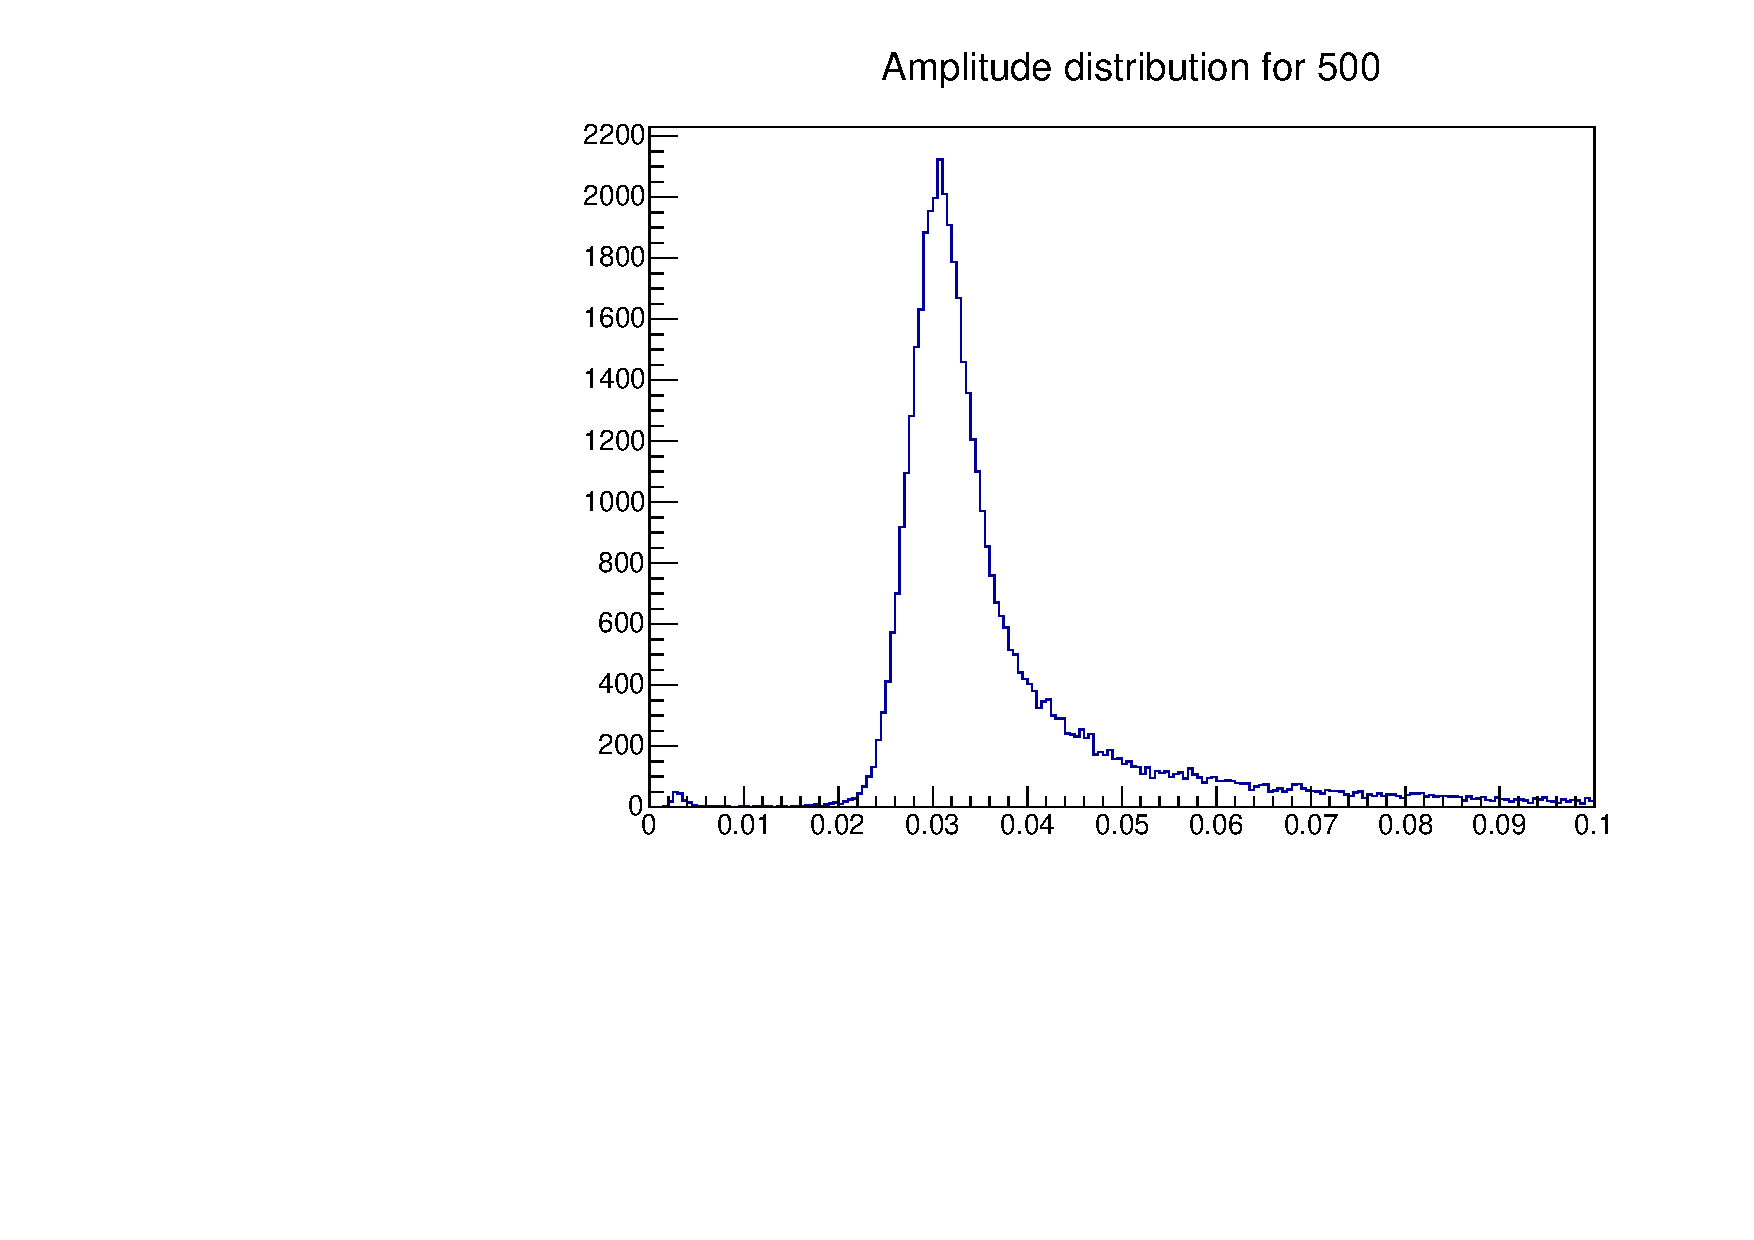
\includegraphics[width=0.6\textwidth]{scripts/pics/S37_500}
\caption{An example of a landau distribution acquired by S37 at 500~V bias voltage PLACEHOLDER}
\label{fig:landausample}
\end{center}
\end{figure}
The resulting CCD for the three measured samples at bias voltages ranging from 0.2--1.0~V~$\upmu$m$^{-1}$ is shown in figure~\ref{fig:ccd}. S37 exhibits full collection distance already at 0.4~V~$\upmu$m$^{-1}$ whereas the irradiated samples have a more gentle increase of CCD with increasing bias voltage. It is evident that at 1~V~$\upmu$m$^{-1}$  the maximum CCD has not been reached in the case of S79 and S52.


\subsubsection{Irradiation damage factor}
The irradiation damage factor $k$ is a way to quantify irradiation damage of a specific particle at a specific energy. Via this factor different types of irradiation can be compared. It is obtained experimentally by measuring the CCD of a number of samples at various irradiation steps and fitting the function~\ref{eq:radfactor1} to the data. $\lambda$ is the measured CCD, $\lambda_0$ is the CCD of a non-irradiated sample and $\Phi$ the radiation dose.
\begin{equation}
\label{eq:radfactor}
\frac{1}{\lambda} = \frac{1}{\lambda_0}+\frac{k}{\Phi}
\end{equation} 
\begin{equation}
\label{eq:radfactor1}
\lambda = \frac{\lambda_0}{k \lambda_0 \Phi + 1}
\end{equation} 

The data points with the maximum CCD obtained in the test beam measurements were plotted against radiation dose received (see figure~\ref{fig:radfactor}). Function~\ref{eq:radfactor1} was fitted to the data points and a damage factor $k=6.2\times 10{-18}$ was obtained. This is three times higher than the damage factor obtained by RD42. A possible cause is that the irradiated samples did not yet have a full charge collection at 1~V~$\upmu$m$^{-1}$.

% CCD against HV 
\begin{figure}[!ht]
%\centering
\begin{tabular}{cccc}
\subfloat[CCD for S37, S79 and S52]{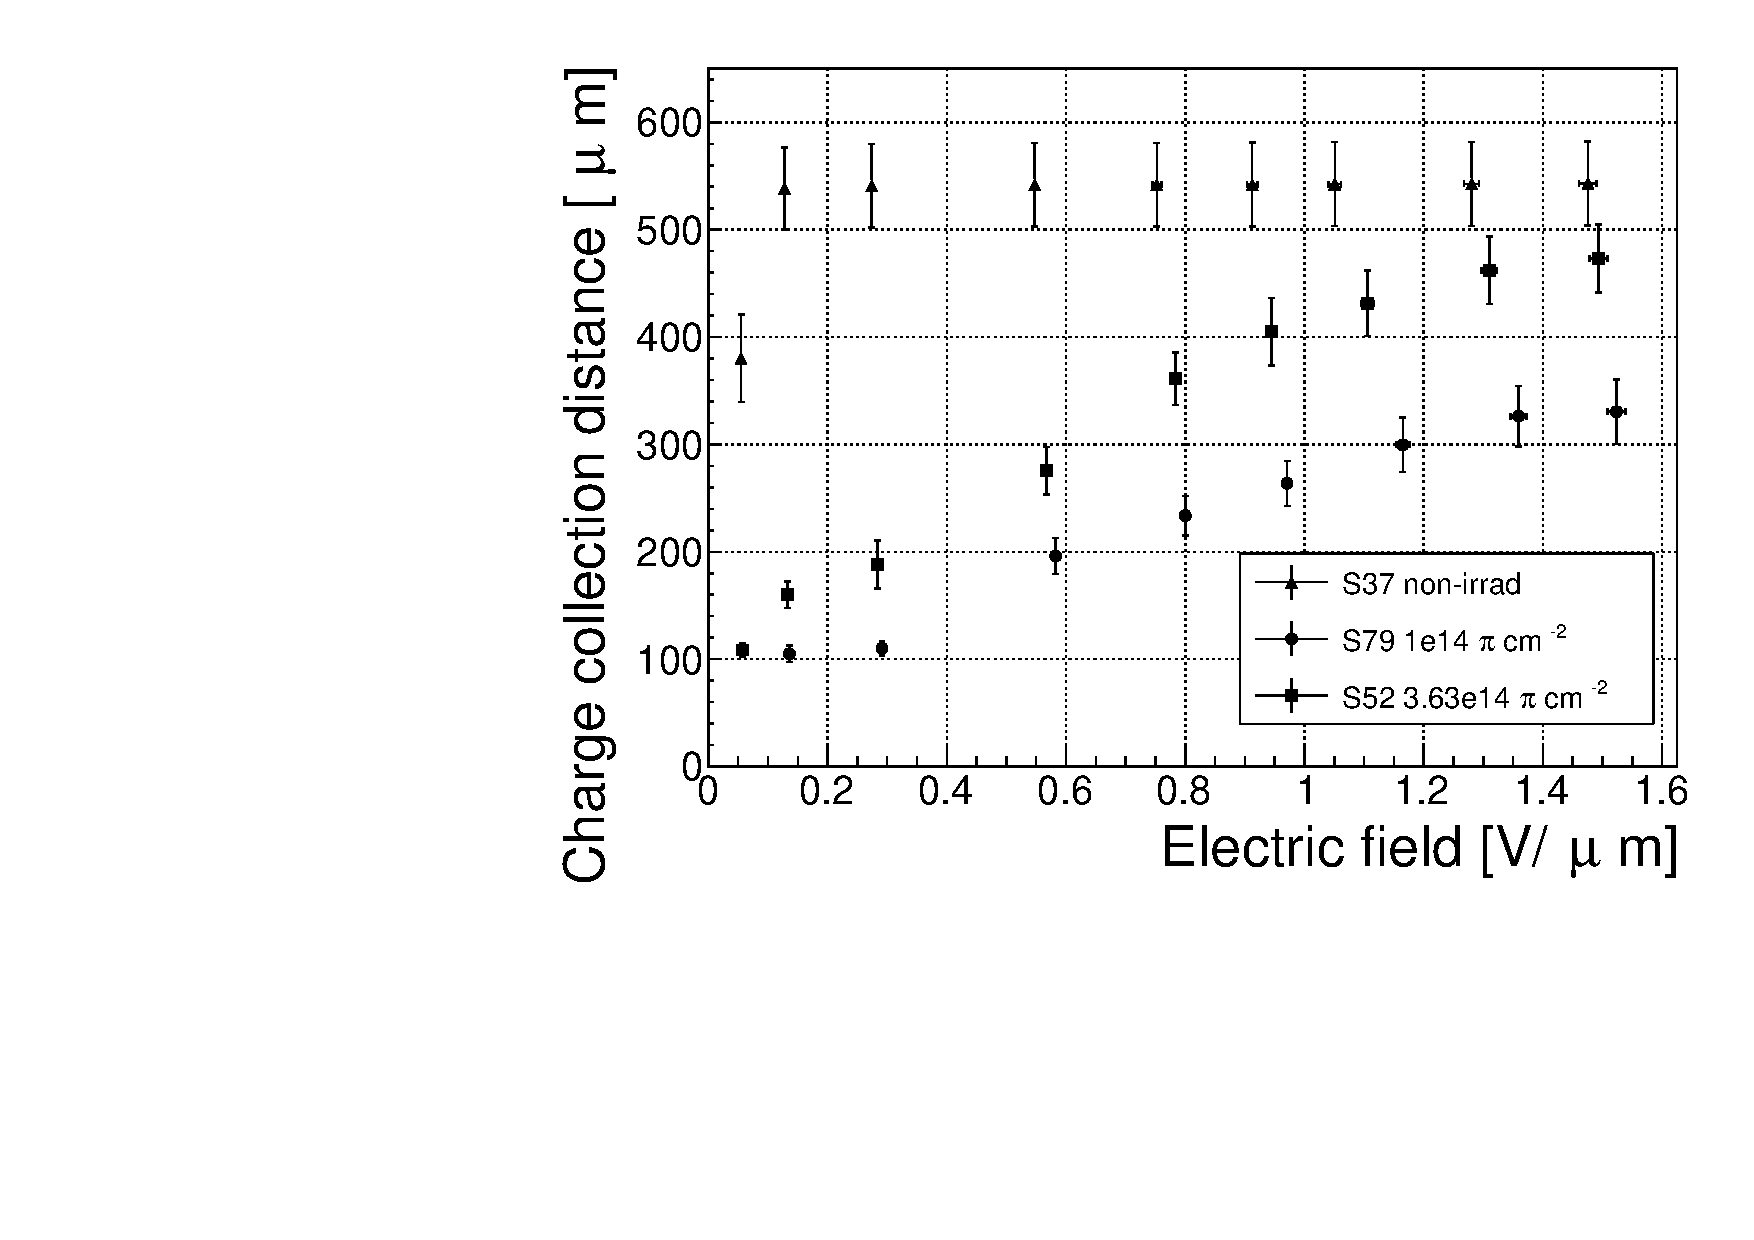
\includegraphics[width=0.45\textwidth]{scripts/plots/ccd} \label{fig:ccd}} &
\subfloat[Comparing the data points obtained in a test beam against the RD42 data]{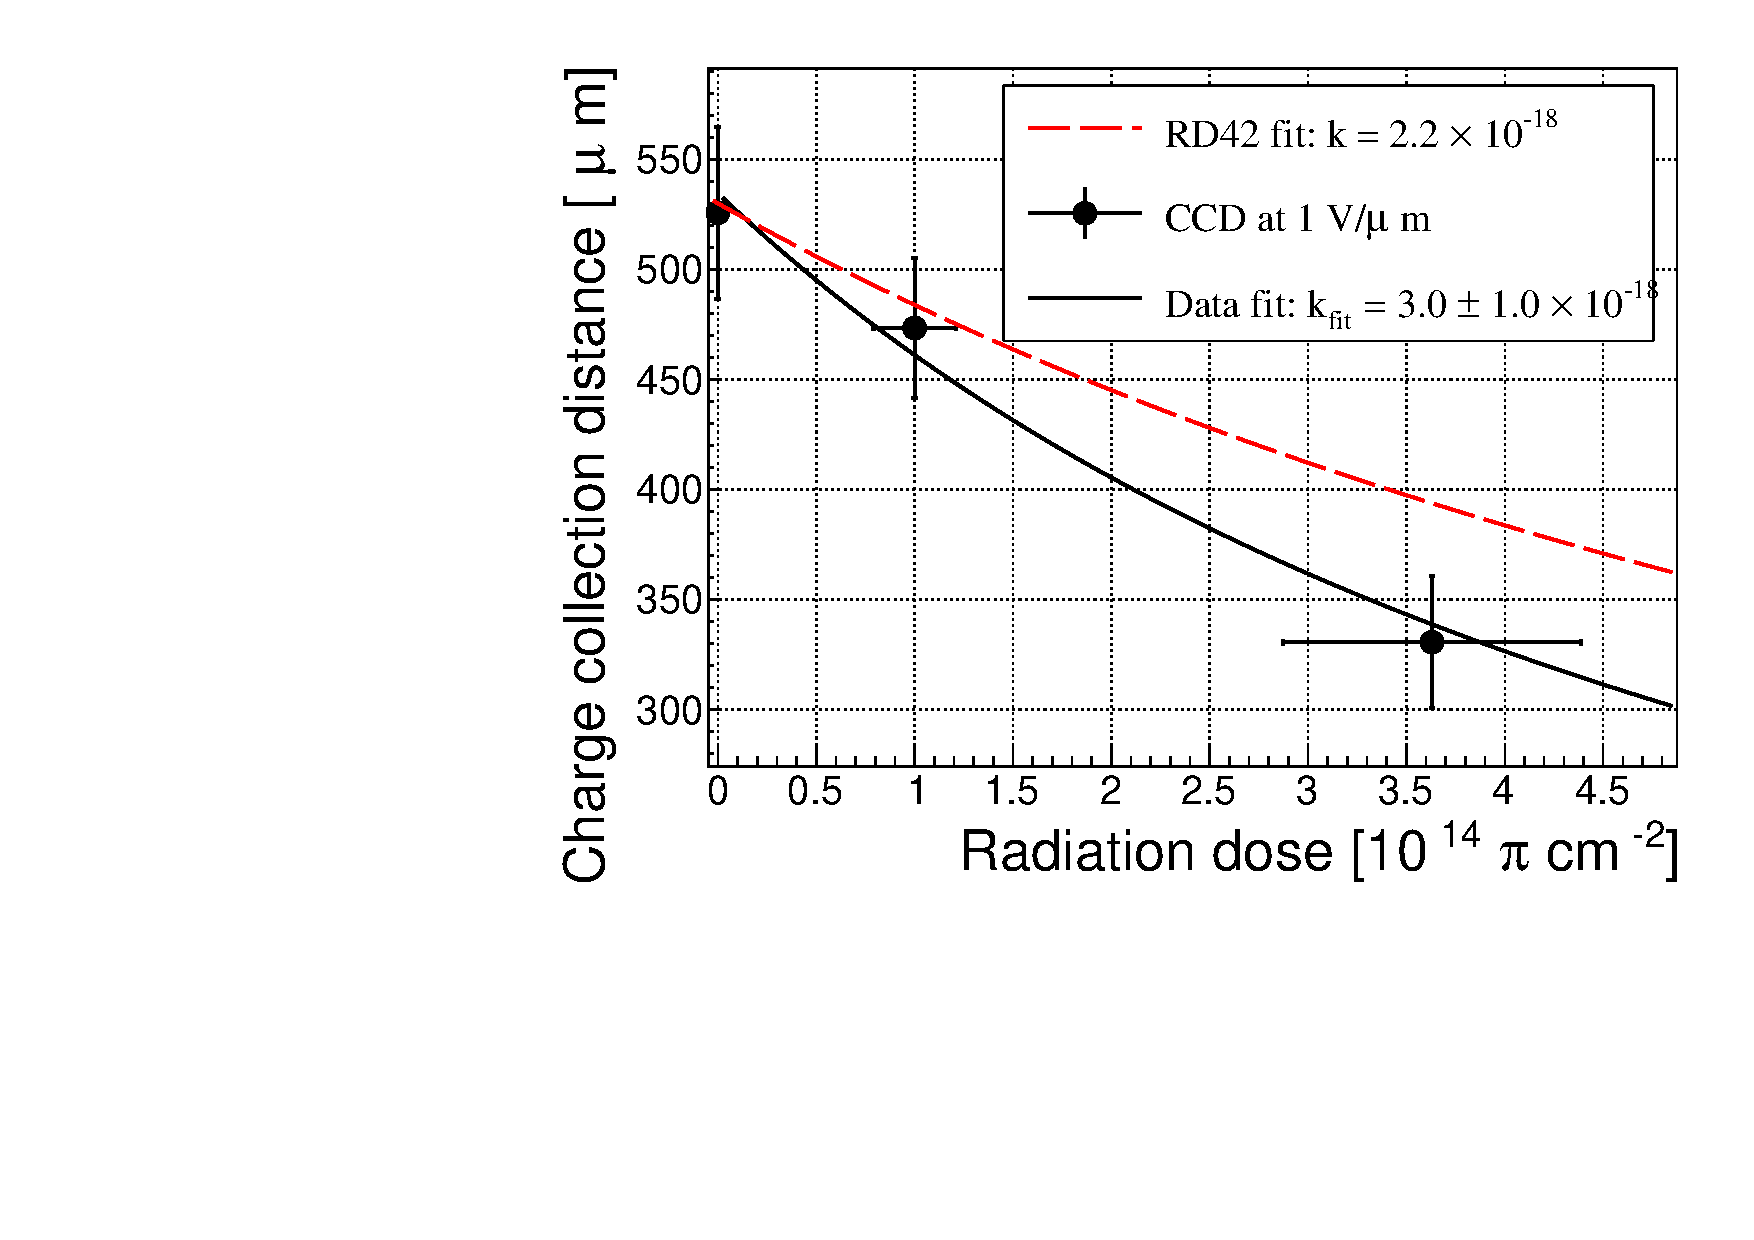
\includegraphics[width=0.45\textwidth]{scripts/plots/radfactor}  \label{fig:radfactor}}
\end{tabular}
\caption{The charge collection distance at 500~V bias voltage for the three diamond samples was compared to the RD42 data for pion irradiation. The data points are not in accordance with the model.}
\end{figure}



\subsection{TCT at room temperature}


\subsubsection{Long-term charge collection stability}
TO-DO: Ramp up to 500 V, take 100 samples every 5 minutes.

The three samples were tested for a long term stability of the current pulse shapes. 
% sample landau distribution  
\begin{figure}[!ht]
\begin{center}
%\includegraphics[width=0.6\textwidth]{}
\caption{Change of the pulse shape with time. PLACEHOLDER}
\label{fig:landausample}
\end{center}
\end{figure}


\subsubsection{Charge collection hysteresis}

\begin{figure}[!ht]
\begin{center}
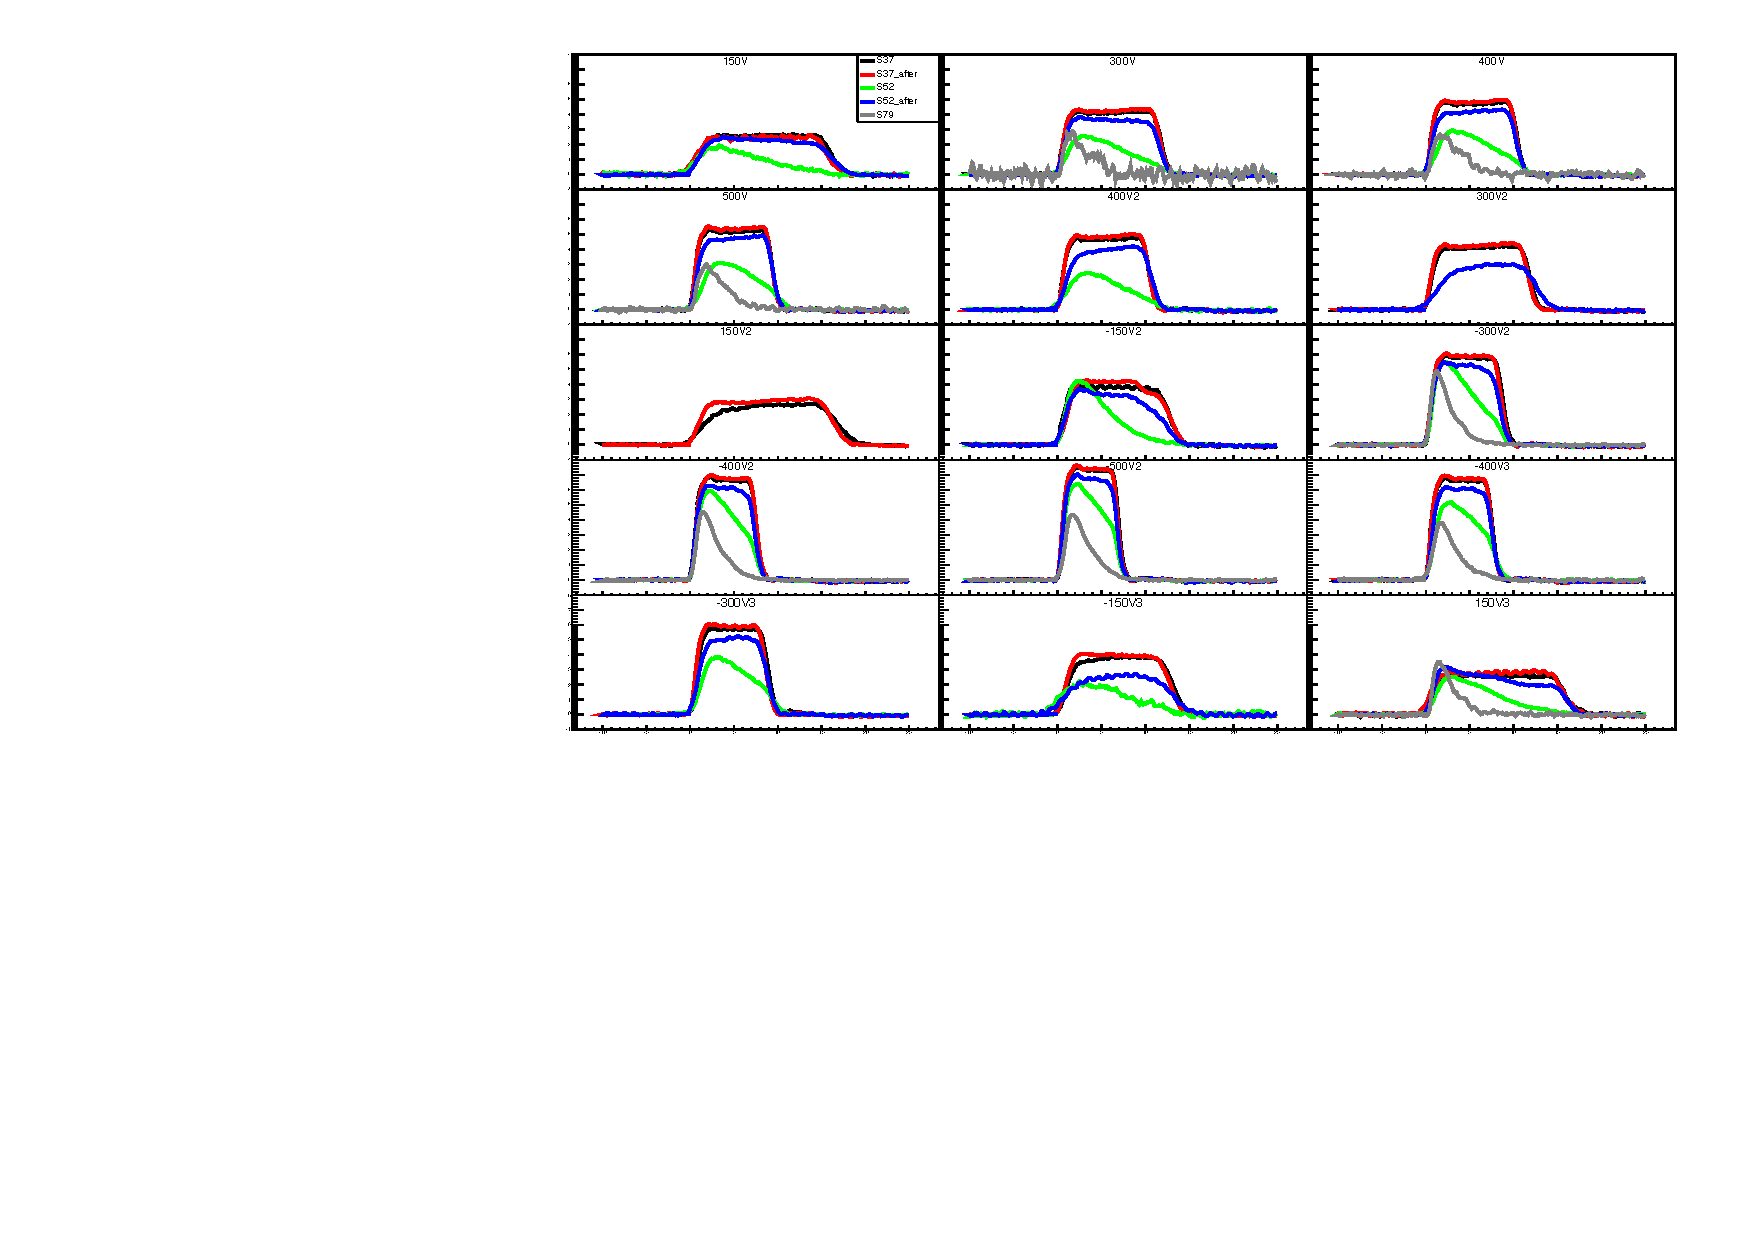
\includegraphics[width=1\textwidth]{plots/hysteresis/all_pulses_1}
\caption{S37 non-irrad; S52 $1\times10^{14}~p~cm^{-2}$ non-pumped, pumped; S79 $3.63\times10^{14}~p~cm^{-2}$ non-pumped, pumped PLACEHOLDER}
\label{fig:hystall}
\end{center}
\end{figure}





\subsection{Temperature-variant TCT}
The irradiated samples were put in the cryostat, which was cooled down to 4.2~K using liquid helium. TCT data were then taken at a range of bias voltages at temperature points ranging between 4.2~K and room temperature (RT). The results showed that irradiation causes forming of charge traps in the bulk.l;'

TO-DO: get the Tau and plot it against T. 
TO-DO: plot the drift time against square voltage.













\section{Conclusion}
\label{sec:radlimit}



% ---------------------------- comment out when compiling the full document -------------------
\end{document}
% ---------------------------------------------------------------------------------------------------------------
